\documentclass[12pt]{article}
%\usepackage{fullpage}
\usepackage{graphicx}
\usepackage{pgfplots}
\usepackage{hyperref}
\usepackage{tikz}
\usepackage{subfig}
\usepackage{showframe}
\begin{document}
\definecolor{tempcolor}{RGB}{124,252,0}

\begin{figure}[h!]
\centering
\subfloat[AAAA]{\label{fig:AAAA}

\begin{tikzpicture}
 \matrix [draw,below left] at (-5,0) {
  \node [fill, circle,fill=red, line width=0mm, inner sep=0pt, minimum size=.5cm, node distance=1.75cm,label=right:Phish/Hack] {}; &
  \node [fill, circle,fill=green, line width=0mm, inner sep=0pt, minimum size=.5cm, node distance=1.75cm,label=right:Token Contract] {}; &
  \node [fill, circle,fill= blue, line width=0mm, inner sep=0pt, minimum size=.5cm, node distance=1.75cm,label=right:Exchange Deposit] {}; &
  \node [fill, circle,fill= yellow, line width=0mm, inner sep=0pt, minimum size=.5cm, node distance=1.75cm,label=right:Exchange Root] {}; \\
  \node [fill, circle,fill= cyan, line width=0mm, inner sep=0pt, minimum size=.5cm, node distance=1.75cm,label=right:Pool] {}; &
  \node [fill, circle,fill= magenta, line width=0mm, inner sep=0pt, minimum size=.5cm, node distance=1.75cm,label=right:Miner] {}; &
  \node [fill, circle,fill=orange, line width=0mm, inner sep=0pt, minimum size=.5cm, node distance=1.75cm,label=right:Investor] {}; &
  \node [fill, circle,fill= tempcolor, line width=0mm, inner sep=0pt, minimum size=.5cm, node distance=1.75cm,label=right:ICO Wallet] {}; 
  
  
  \\
};


\end{tikzpicture}

}%
\hfill 
\subfloat[BBBB]{\label{fig:BBBB}
\resizebox{6.5cm}{!}{
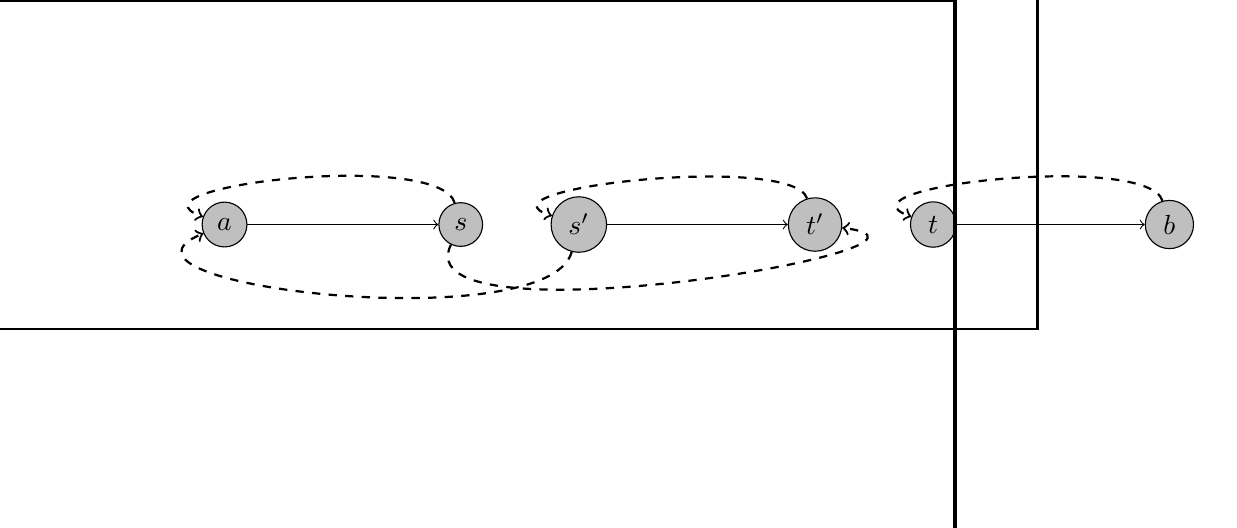
\begin{tikzpicture}[every node/.style={circle, draw, scale=1.0, fill=gray!50}, scale=1.0, rotate = 180, xscale = -1]
\node (1) at (0, 0) {$a$};
\node (2) at (3.0, 0) {$s$};
\node (3) at (4.5, 0) {$s'$};
\node (4) at (7.5, 0) {$t'$};
\node (5) at (9.0, 0) {$t$};
\node (6) at (12.0, 0) {$b$};
\draw[->] (1) -- (2);
\draw[thick, dashed, ->] (2) to[out=-100,in=-150] (1);
%%\draw (3) -- (2);
\draw[->] (3) -- (4);
\draw[thick, dashed, ->] (4) to[out=-100,in=-150] (3);
%%\draw (5) -- (4);
\draw[thick, dashed, ->] (2) to[out=-250,in=-350] (4);
\draw[thick, dashed, ->] (3) to[out=100,in=150] (1);    
%%\draw (8) -- (7);
\draw[->] (5) -- (6);
\draw[thick, dashed, ->] (6) to[out=-100,in=-150] (5);
\path[step=1.0,black,thin,xshift=0.5cm,yshift=0.5cm] (-3,-3) grid (12,3);
\end{tikzpicture}
}
}%
\hfill 
\subfloat[CCCC]{\label{fig:CCCC}
\resizebox{6.5cm}{!}{
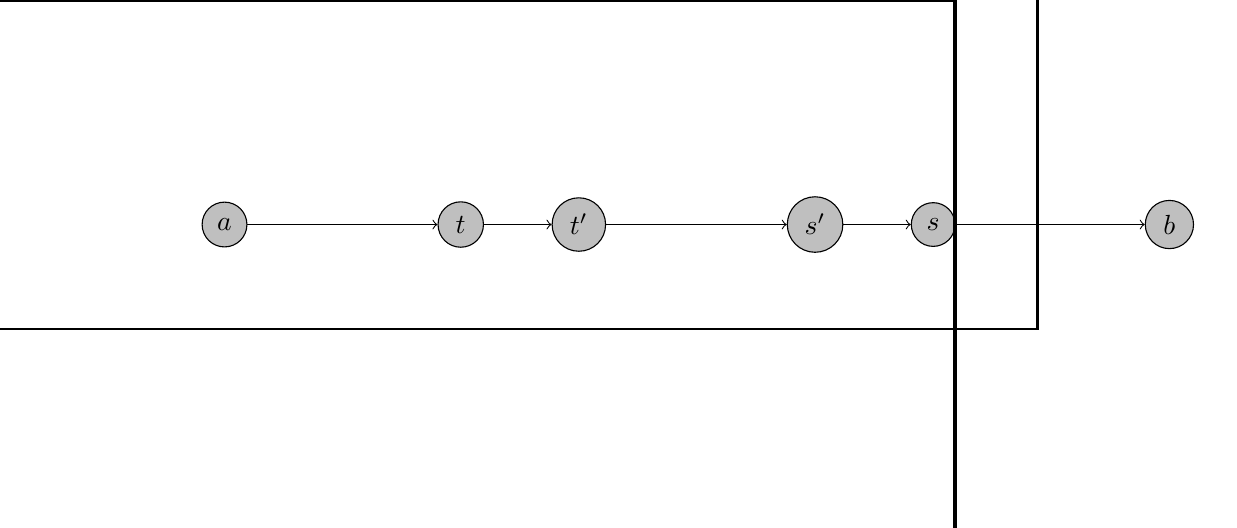
\begin{tikzpicture}[every node/.style={circle, draw, scale=1.0, fill=gray!50}, scale=1.0, rotate = 180, xscale = -1]
\node (1) at (0, 0) {$a$};
\node (2) at (3.0, 0) {$t$};
\node (3) at (4.5, 0) {$t'$};
\node (4) at (7.5, 0) {$s'$};
\node (5) at (9.0, 0) {$s$};
\node (6) at (12.0, 0) {$b$};
\draw[->] (1) -- (2);
\draw[->] (2) -- (3);
\draw[->] (3) -- (4);
\draw[->] (4) -- (5);
%%\draw (8) -- (7);
\draw[->] (5) -- (6);
\path[step=1.0,black,thin,xshift=0.5cm,yshift=0.5cm] (-3,-3) grid (12,3);
\end{tikzpicture}
}
}%
\hfill 
\subfloat[DDDD]{\label{fig:DDDD}
\resizebox{6.5cm}{!}{
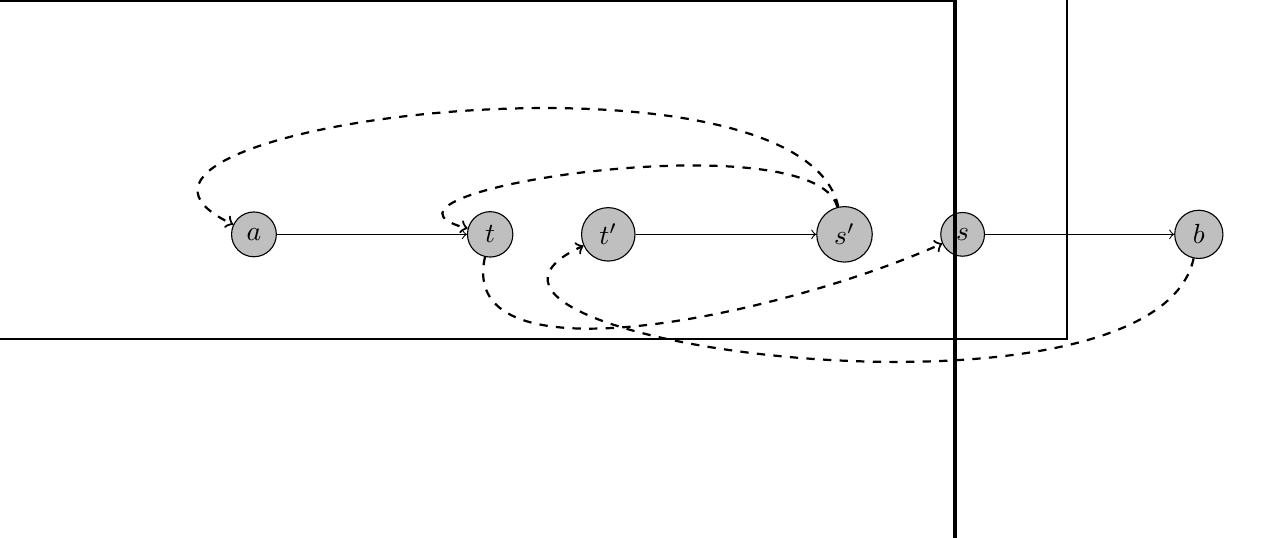
\begin{tikzpicture}[every node/.style={circle, draw, scale=1.0, fill=gray!50}, scale=1.0, rotate = 180, xscale = -1]
\node (1) at (0, 0) {$a$};
\node (2) at (3.0, 0) {$t$};
\node (3) at (4.5, 0) {$t'$};
\node (4) at (7.5, 0) {$s'$};
\node (5) at (9.0, 0) {$s$};
\node (6) at (12.0, 0) {$b$};
\draw[->] (1) -- (2);
\draw[thick, dashed, ->] (4) to[out=-100,in=-150] (1);
%%\draw (3) -- (2);
\draw[->] (3) -- (4);
%\draw[thick, dashed, ->] (5) to[out=100,in=150] (1);
%%\draw (5) -- (4);
\draw[thick, dashed, ->] (2) to[out=100,in=150] (5);
\draw[thick, dashed, ->] (4) to[out=-100,in=-160] (2);  
%%\draw (8) -- (7);
\draw[->] (5) -- (6);
\draw[thick, dashed, ->] (6) to[out=100,in=150] (3);
\path[step=1.0,black,thin,xshift=0.5cm,yshift=0.5cm] (-3,-3) grid (12,3);
\end{tikzpicture}
}
}%
\hfill 
\caption{Aligning figures in a table}\label{fig:FIGone}
\end{figure}
\end{document}